% !TEX encoding = UTF-8
% !TEX TS-program = pdflatex
% !TEX root = ../tesi.tex

%**************************************************************
\chapter{Web Service e Database}
\label{cap:sviluppo-software}
%**************************************************************

In questo capitolo sono trattati gli elementi di base delle soluzioni sviluppate. In primo luogo sono illustrati i Web Service, responsabili della maggior parte delle operazioni. Successivamente è mostrato il Database di supporto con le principali caratteristiche.


%**************************************************************
\section{Web Service}

Secondo la definizione del (GLOSSARIO)World Wide Web Consortium (W3C), un Web Service è un sistema software progettato per supportare l'interoperabilità tra diversi elaboratori su di una medesima rete.
Questa caratteristica si ottiene associando all'applicazione un'interfaccia Software che espone all'esterno i propri servizi, per mezzo della quale altri sistemi possono interagire con l'applicazione stessa utilizzando le operazioni descritte nell'interfaccia. L'utilizzo delle operazione avviene tramite richieste, nel caso in esame di tipo SOAP (approfondito nella sezione \ref{soap}). I messaggi di richiesta sono formattati secondo lo standard XML, incapsulati e trasportati tramite protocollo HTTPS. 
La connessione implementa il protocollo HTTPS, invece del classico HTTP, per aumentare la sicurezza del sistema, poiché trattandosi di dati riservati un utente malintenzionato vorrebbe poter disturbare la connessione o manometterne i dati trasmessi.\\
Grazie anche all'utilizzo di standard basati su XML, un'architettura basata su Web Service permette ad applicazioni software scritte in diversi linguaggi di programmazione e implementate su diverse piattaforme hardware di utilizzare le funzionalità che essa espone senza difficoltà.
\\Nella Figura \ref{webservice} è mostrato, in modo semplice, il funzionamento di un Web Service.

\begin{figure}[!h] 
    \centering 
    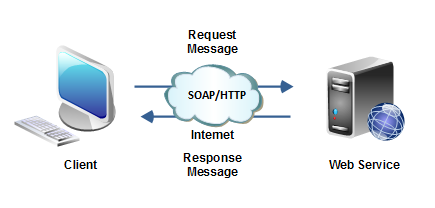
\includegraphics[width=0.60\columnwidth]{web-service} 
    \caption{Funzionamento di un Web Service}
    \label{webservice}
\end{figure}


Nella realizzazione delle soluzioni sono stati sviluppati tre Web Service,\\ \texttt{LicenseManagerService}, \texttt{LicenseEmailService} e \texttt{LicenseSecurityService}, spiegati nei paragrafi successivi. Ognuno di essi è responsabile di funzionalità ben precise e sono indipendenti tra di loro per fornire un grado più alto di affidabilità ed eliminare le dipendenze.


\subsection{Richieste SOAP}
\label{soap}
SOAP, acronimo di \textit{Simple Object Access Protocol}, è un protocollo per lo scambio di messaggi tra componenti software, nel caso in esame tra Client e Web Service, che avviene per mezzo della sintassi XML. \\
Il protocollo definisce un insieme di regole che il Client deve rispettare per richiedere al server che ospita ed espone il Web Service una determinata operazione.
\\
Un messaggio SOAP è formato da un \texttt{Header} e da un \texttt{Body}:
\begin{itemize}
\item \textbf{Header:} è facoltativo e contiene meta-informazioni, come ad esempio informazioni di sicurezza o parametri per eseguire una procedura;
\item \textbf{Body:} è obbligatorio e contiene il contenuto del messaggio, strutturando secondo (GLOSSARIO)l'XML Schema imposto dal Web Service.
\end{itemize}

Nella Figura \ref{soap} è mostrato un esempio di richiesta e risposta del metodo \texttt{setEmail} del Web Service \texttt{LicenseEmailService}.

\begin{figure}[!h] 
    \centering 
    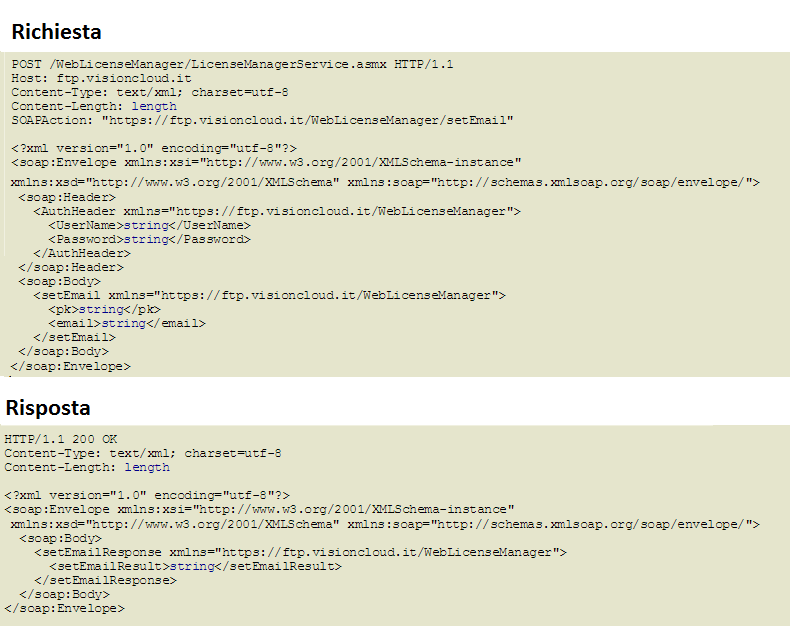
\includegraphics[width=1\columnwidth]{soap} 
    \caption{Esempio di richiesta e risposta SOAP}
    \label{soap}
\end{figure}

Come si può vedere dalla Figura \ref{soap}, l'\texttt{Header} delle richieste è stato definito in modo da implementare un sistema
di autenticazione, per far sì che i Web Service siano utilizzati esclusivamente da Client autorizzati. Questo argomento è illustrato in dettaglio nel prossimo paragrafo.

\subsection{Autenticazione}

\subsection{LicenseManagerService}

\subsection{LicenseEmailService}

\subsection{LicenseSecurityService}


%**************************************************************
\section{Database - DBLicenze}
\label{sez:DBLic}
elenco tabelle con caratteristiche generali
